\section{State Space Controller Implementation}\label{sec:SSImplementation}
The controller in state space results to be three gains that do not need to be discretized to implement them in the real system. Listing \ref{codeStateSpaceControl} contains the code for the function that calculates the action of control.
\lstinline[style=customcppinline]{x_hat} contains the states of the system, being the angle of the frame (\lstinline[style=customcppinline]{x_hat[0]}), the velocity of the frame (\lstinline[style=customcppinline]{x_hat[1]}) and the velocity of the wheel (\lstinline[style=customcppinline]{x_hat[2]}). \lstinline[style=customcppinline]{x_hat} is the equivalent of vector \si{\vec{x}}. The inner product between \si{\vec{K}} and \si{\vec{x}} is calculated on line 11 in code listing \ref{codeStateSpaceControl}. On line 14 the found output torque is converted to a current, since the motor control board takes a current as reference. The \lstinline[style=customcppinline]{TORQUE_2_CURRENT} constant is found by taking the inverse of the motor torque constant.
\newpage
\begin{lstlisting}[style = customcpp,
                  caption  = {Code for the implementation of the State Space Controller. The feedback from the Cubli is contained in the array x\_hat.},
                  label    = codeStateSpaceControl ]
/** Runs the controller based on the feedback signal in x_hat */
LSF_COutput_struct_T AAU3_DiscLinFeedback2(const real_T x_hat[3])
{
/** Variable declarations */
LSF_COutput_struct_T LSF_Sig_Out;

/** Controller calculations */
LSF_Controller.tau_m = 0;
for (int i = 0; i < 3; i++)
{
LSF_Controller.tau_m += LSF_Controller.K[i] * x_hat[i];
}

LSF_Sig_Out.I_m = LSF_Controller.tau_m * TORQUE_2_CURRENT;

return LSF_Sig_Out;
}
\end{lstlisting}
The important part of the implementation, and in some cases it can give problems, is the measurement of the states that are involved in the feedback.
In the case of the Cubli, there are three states to be measured: the position and velocity of the frame and the velocity of the wheel.

The first one can be measured using the values from the potentiometer or using built-in sensors like the IMU, as will be explained in detail in \chapref{chap:CompFilter}.

The velocity of the frame is measured using the gyroscopes present in both IMUs, which give an angular velocity value.

Finally, information about the velocity of the wheel is measured with a tachometer attached to the motor and send to the BeagleBone through the motor control board. 
\\
\begin{figure}[H]\vspace{-4mm}
	\centering
	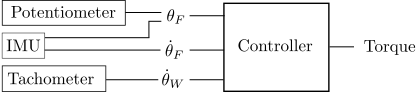
\includegraphics[scale=.75]{figures/measurements}
	\captionof{figure}{Internal states measurements for the implementation of the controller.}
	\label{fig:measurements}
\end{figure}\vspace{-5mm}
